\documentclass{article}
\usepackage{enumitem}
\usepackage[a4paper, total={6in, 8in}, margin=1in]{geometry}
\usepackage{graphicx}
\newcommand*{\ttt}[1]{\texttt{#1}}
\graphicspath{{./res/}}

\begin{document}
\section{Design Overview}
\subsection{Files}
\begin{enumerate}
    \item \texttt{storage.cpp}
    \subitem{
        This file defines the structure for each storage nodes in the homogeneous structure that powers this distributed file system.
    } 
    \item \texttt{client.cpp}
    \subitem{
        This class abstracts interactions with the manager for the user.
    }
    \item \texttt{manager.cpp}
    \subitem{
        This class is in charge of managing each storage node. Client nodes contact the server before making any GET or PUT requests to client nodes. 
    }
\end{enumerate}

\section{Storage Components}
\subsection{Sockets}
Each node (client, manager, storage) exposes a unique port that can be connected to by multiple processes.
This is the "listen" port. For the manager class, this port is static and can only be configured before runtime.
For the other nodes, their listen port is randomly chosen by the OS at runtime and it is their responsibility to make the manager aware of their listening port number.
In our case, all nodes are on the same local IP address. However, in the event that nodes are spread out on different machines, the user or daemon starting the storage and client
nodes would be responsible for knowing which IP address the manager is on, and the code would be edited to take in a command line input to set the manager IP address
they would be connecting to. The discovery message the storage node sends to the manager would also be changed to contain a return ip address in addition to a return port.
This information would also need to passed to the client when giving out primary nodes to connect to, and to storage nodes when passing out replica information.


\subsection{Packet Types}
There are multiple types of packets in our architecture but each type begins with a \texttt{uint\_8} header describing the packet type for easy parsing.

The packet types are as follows
\begin{enumerate}
    \item \texttt{DISC}
    \subitem used for storage node initialization. This is how the manager discovers the children.
    \item \texttt{PUT}
    \subitem used when a client or storage node wants to store a key
    \item \texttt{GET}
    \subitem used when a client wishes to recieve a value at a given key
    \item \texttt{ACKPUT}
    \subitem response given by storage node when PUT was successful
    \item \texttt{ACKGET}
    \subitem response given by storage node when GET was successful
    \item \texttt{FAIL}
    \subitem General Failure message sent by storage node or client upon connection timeout. Sent to manager, and contains failing node to purge from the record
    \item \texttt{S\_INIT}
    \subitem and informs them that they are a primary in the event of node 
    failure or system initialization. From a storage nodes perspective, there is no distinction between the two.
\end{enumerate}

\subsection{Storage Node/Initialization}
Storage nodes are initialized separately from the manager daemon.
When a storage node is spawned, it sends a \texttt{DESC} packet to the manager and is added to the pool of available nodes.
Each storage node is apart of a group as determined by the manager.
Groups are assigned ina round robin fashion to ensure a balanced load across all nodes. 
In every group there exists one primary node that is the primary communication device for the client.
The primary within a group is made aware of its neighbors by an \texttt{S\_INIT} packet from the server. If the primary where to die, 
the manager will send a \texttt{S\_INIT} with a new group with the dead node purged to the next replica in line. If a replica where to die,
the manager will update the primary with a new group with the dead node purged with the same message.
\pagebreak
\subsection{Client \texttt{PUT} operation}
When a client wants to store a value at a given key into a node, it first asks the manager for the node group responsible for that key.
The packet sent to the manager has a field for key and a field for value.
The value field is a stringified version of the original vector in which each value is joined by a pipe deliminator.
If that key has yet to be tracked, the server uses round robin to find an available group and assigns it to the given key. This ensures balance among
existing groups.

The client is then given a group struct with the port number for the primary storage node and a list of it's neighbors for redundancy. 
This list is never used directly by the client.

A client then sends the same \texttt{PUT} packet to the primary node and is given a \texttt{ACKPUT} response if successful.

In the background, the primary storage node broadcasts that same packet out to all of it's neighbors. If the client or primary server time out a connection
to a node, it sends a failure connection with the failing port to the manager, which will purge the group of that port. 

A diagram of the program flow is included below:\\

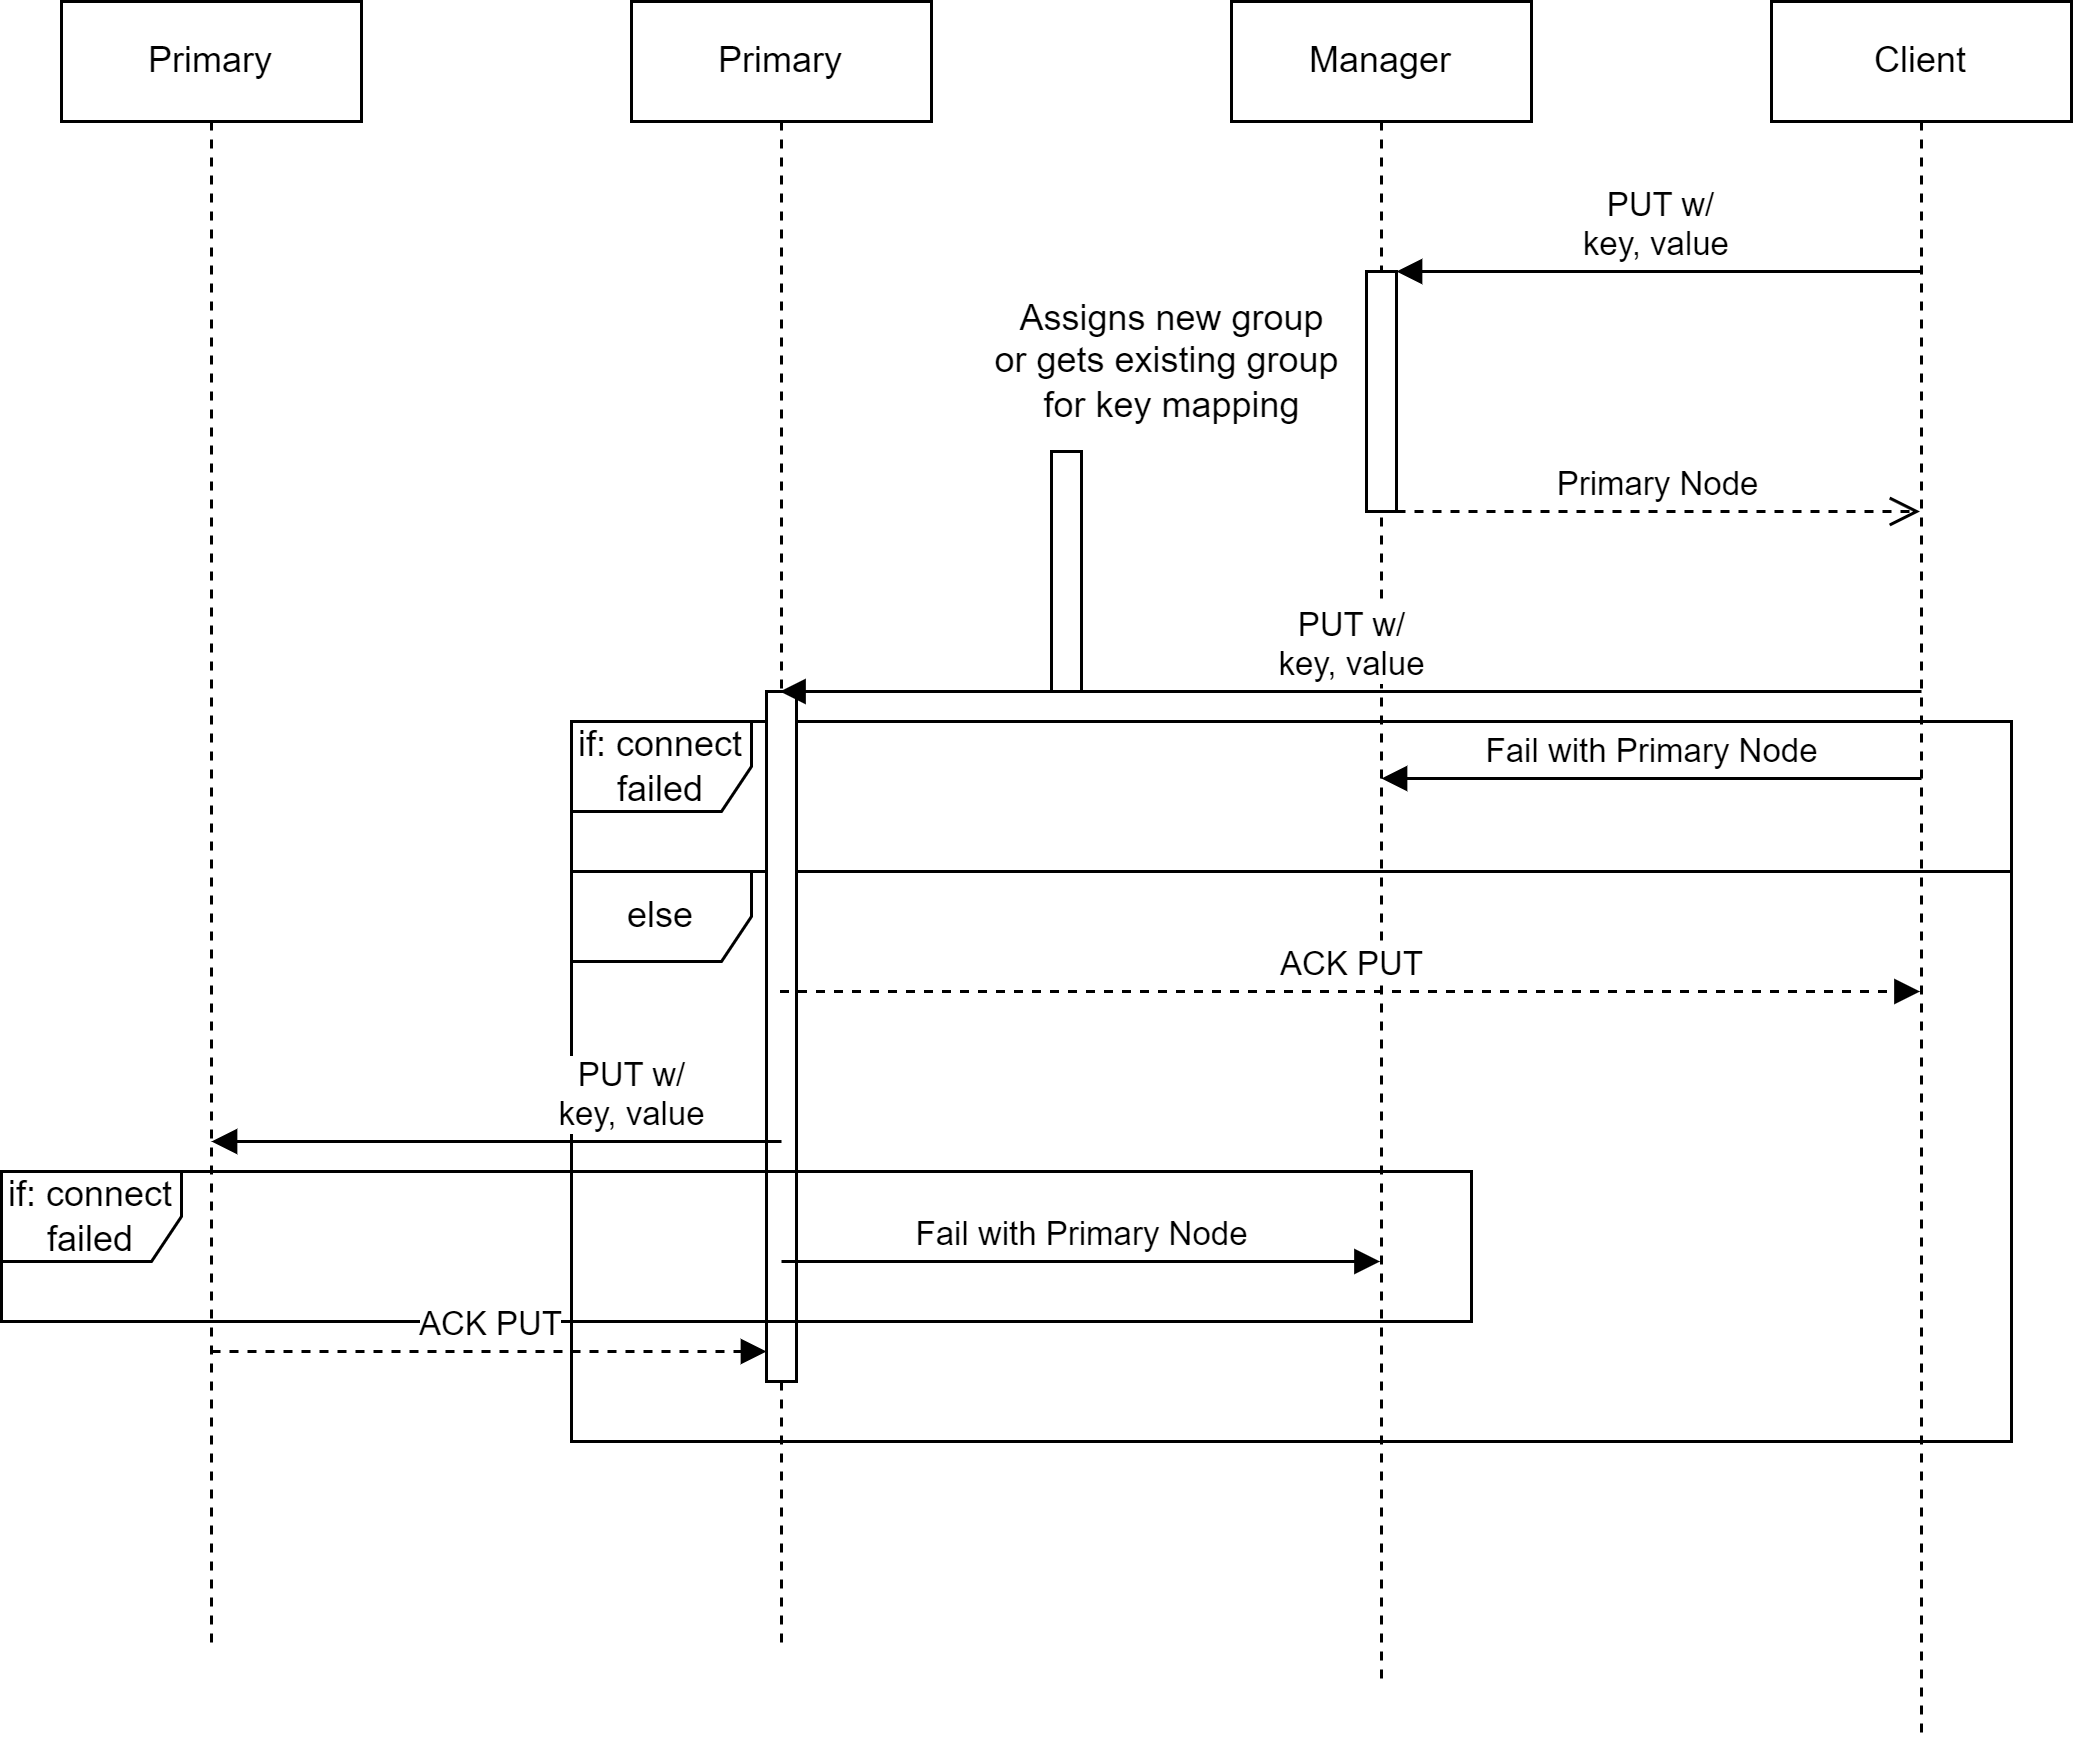
\includegraphics[width=\linewidth]{img/Put.drawio.png}



\pagebreak
\subsection{Client \texttt{GET} operation}
When a client desires a value for a given key, it first asks the manager to find the group responsible for that key.
If that key does not exist in the manager's housekeeping, a generalized \texttt{FAIL} packet is returned. The client should then fail the get request.

If the key does exist, the client is returned a group struct with the port number for the primary storage node and a list of it's neighbors for redundancy. 
Again, this list is never used directly by the client.

The client then forwards the \texttt{GET} packet to the primary node and is given a \texttt{ACKGET} response if successful.

In this packet, the \texttt{value} field is now non-null. 
In it is a string delimitated by |. 
The client library splits this string into substrings based around this deliminator and returns a vector to the original caller.

A diagram of the program flow is included below. Note that because there is no need to contact replicas, 
the flow is significantly less complex:\\
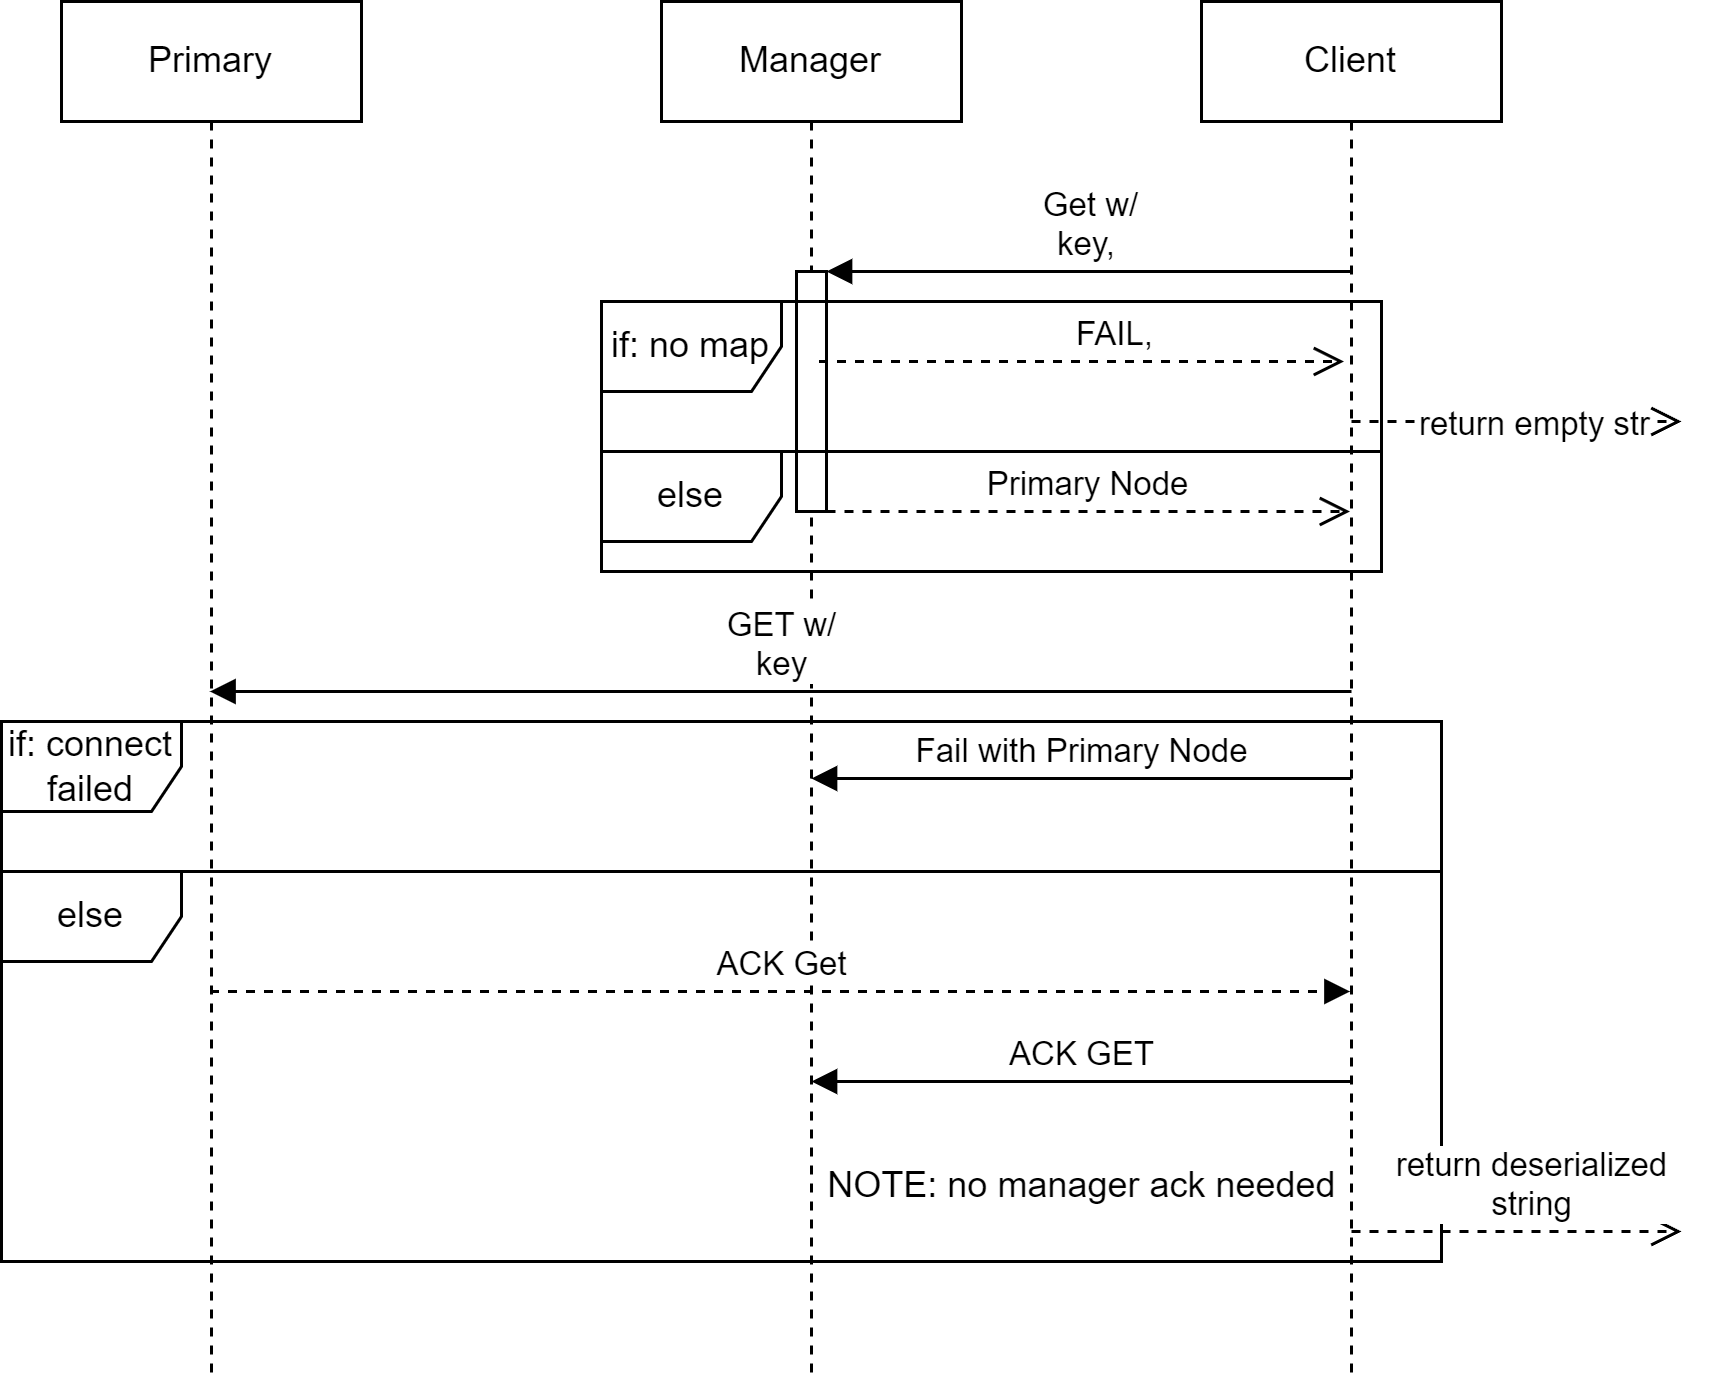
\includegraphics[width=\linewidth]{img/Get.drawio.png}


\subsection{GTStore Manager (Data Partitioning)}
The manager is responsible for assigning and maintaining a an active map of keys to storage groups. It is the first point of contact for any client API call.
The manager's primary function is to return to the client an accurate, up to date port for the key request, regardless of which operation. It is also responsible for updating
groups by purging dead storage nodes in the event of Primary or Client timeouts.

\begin{itemize}
    \item \textbf{\underline{Load Balancing and Group Assignment:}} The manager initially assigns discovered storage nodes to storage groups, where the first node in the group
    is a primary, and the rest are replicas. The manager guarantees each group will have $k$ nodes. In the event that $n \% k != 0$, it will start ``double dipping'' in storage nodes
    to maintain group size. In this way, a single node can belong to both groups, and can be both a primary and a replica. This has load balancing ramifications, which will be discussed below. 
    The manager propagates this info to the primary node. Every time a new key is called, it assigns a group to the key in a round robin fashion. 
    This implements a load balancing scheme where all groups have a comparable amount of keys assigned to them.
    \item \textbf{\underline{Node Failure:}} When a primary or a client fails to connect to a replica or a primary respectively, a \texttt{FAIL} message is sent to the manager. 
    The manager identifies if the failure is a primary or a replica (by where it is in the group, primaries are always the head), and purges it from the group. If the purged
    node is a primary, it assigns a new primary and sends it a \texttt{S\_INIT} packet. If the node is a replica, it sends the existing primary a \texttt{S\_INIT} packet with the 
    new group assignments. 
    \item \textbf{\underline{Load Balencing:}} Because of how we ``double dip'' when allocating groups initially, a single storage node can be a member of two groups at once. Since the 
    round robin scheme of assigning keys to groups only guarantees that a particular group will have the same number of keys, if a node belongs to two groups, it will have double the keys.
    This puts an inordinate amount of strain on this one node. This is unavoidable however, since the project spec requires that a particular group have k nodes. We cannot conjour up nodes
    ourselves, so we are forced to make this compromise. A better solution would be to create an algorithm that would only ever assign a node to a single group, and balance the remaining
    out among the groups that it could. For example, with n=9 and k =4, we would have one group of of five and one group of 4, or even 3 groups of 3. This ensures no node is overburdened
    at the expense of not being able to guarantee group size.
\end{itemize}

\subsection{Data Management}
\begin{enumerate}
    \item manager has key group map
        \subitem PUT: the key map is used to determine if an existing group holds the key. If it does, the manager returns this group. Otherwise, the manager assigns a new group
        with the Round robin scheme discussed above.
        \subitem GET: the key map is used to determine if an existing group holds the key. If it does, the manager returns this group. Otherwise, the manager returns a \texttt{FAIL}
        message as an indication that the client should return an empty string.
    \item each node has a view of what keys it has. Only the primary needs it, but all nodes have it for flexibility.
\end{enumerate}
\subsection{Data Redundancy}
The primary is responsible for propagating data to its replicas. This ensures that there are copies of any given put in the system. Once a client fails to connect to a primary,
it notifies the manager and a new primary is assigned to take the old one's place. After all primaries in the group have been exhausted, the manager will fail out, as per the project
specs. 
\subsection{Node Failure}
\begin{enumerate}
    \item We do not use a heartbeat. This only serves to clog the manager with addition messages that perform a redundant operation that a client or primary storage node timeout
    serves to indicate. All a heartbeat serves to do is to ensure that the manager can self-discover failed nodes. This requires it to timeout on every node it sends a heart beat too.
    Since a socket can only connect to a single node, we must open N sockets, likely in N threads, to perform a polling operation. Our scheme performs the same functionality but does it
    in a greedy fashion. It only handles node failures when it NEEDS to. This results in less complexity and overhead for the manager at the expense of marginal performance gains on the 
    client side. The scenario in which the heartbeat would benefit the manager is when a node dies when a client has not attempted to interact with it for a long time. This heartbeat 
    ensures that the next time the client tries to access that particular storage group, the manager will provide up to date information. However, this situation is relatively rare, and 
    we would still need to handle the case in which the primary node dies in between the time when a heartbeat occurs and a manager sends a group to the client. Considering all of these factors
    combined, we decide to not use a heartbeat to discover dead nodes. 
    \item There are two cases of node failures: primary node death and replica node death. When a primary dies, it will be discovered by the client trying to perform an action. This is 
    handled by sending a \texttt{FAIL} message to the manager, and the manager performing the necessary primary reassignment discussed above. The next is replica death. From the perspective
    of the client, replica death has no ramification to expected behavior. The client still receives the queried value or puts the requested value on the primary group. This is why
    the primary sends an ack back to the client BEFORE it begins propagation to its replicas. The client simply does not care. The primary then sends a \texttt{PUT} message to each of 
    its replicas and sends a \texttt{FAIL} message to the manager for each node that fails. The manager performs the necessary purging, as does the primary to maintain consistent lists.
\end{enumerate}

\subsection{Data Consistency}
Data consistency is maintained through replication. A node that fails a connection during replication for any reason is considered dead, even if it restarts on the same address later.
This ensures that nodes within a group have consistent data. Since the client contacts the storage nodes directly, there is no need to keep data consistent from a manager, storage node
perspective. In fact, the manager does not even store values, or use the value field in a put message in any way. Storage nodes are the only nodes to ever handle the actual storage of data.
\section{Results}


\subsection{Performance}
Below are the performance benchmarks test runs for 7 nodes, 1, 3 and 5 replicas, in order:\\\\
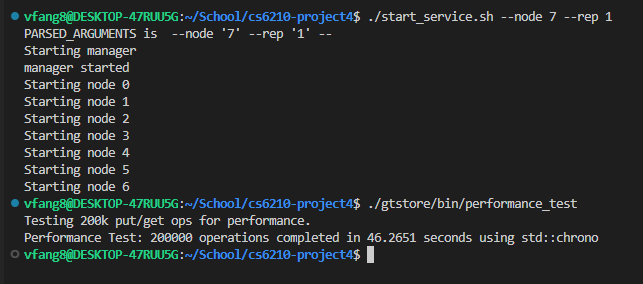
\includegraphics[width=\linewidth]{img/Performance71.png}\\
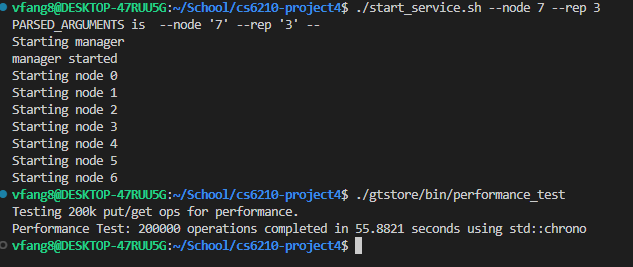
\includegraphics[width=\linewidth]{img/Performance73.png}\\
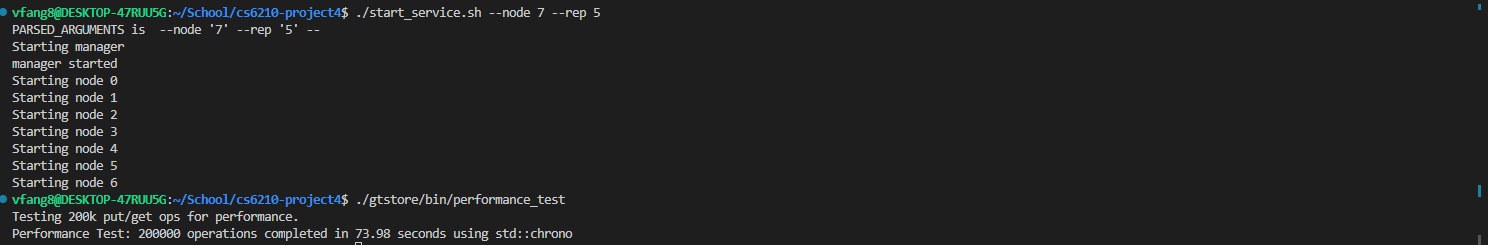
\includegraphics[width=\linewidth]{img/Performance75.png}\\\\
We can see a stead linear increase in runtime. As replica counts increase, the number of actual put ops will expand to \texttt{client_ops * k}, because each 
client op must be replicated accross k nodes. Obviously, we do not experience this in get ops, but the 100k put ops will take longer. This will manifest itself 
as a linear increase in time per op.\\\\
Below is a line graph of the results:\\\\
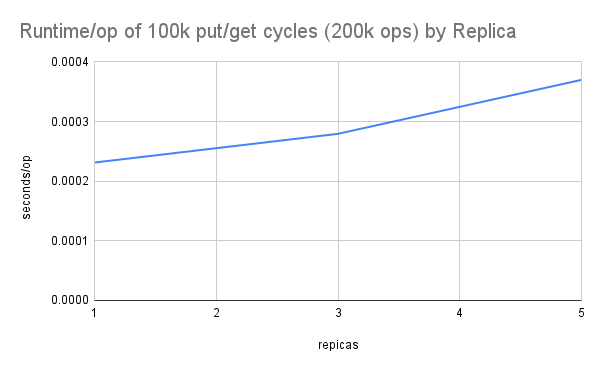
\includegraphics[width=\linewidth]{img/PerformanceChart.png} 

\pagebreak
\subsection{Load Balancing}
Below is the last few lines of the load benchmark run:\\\\
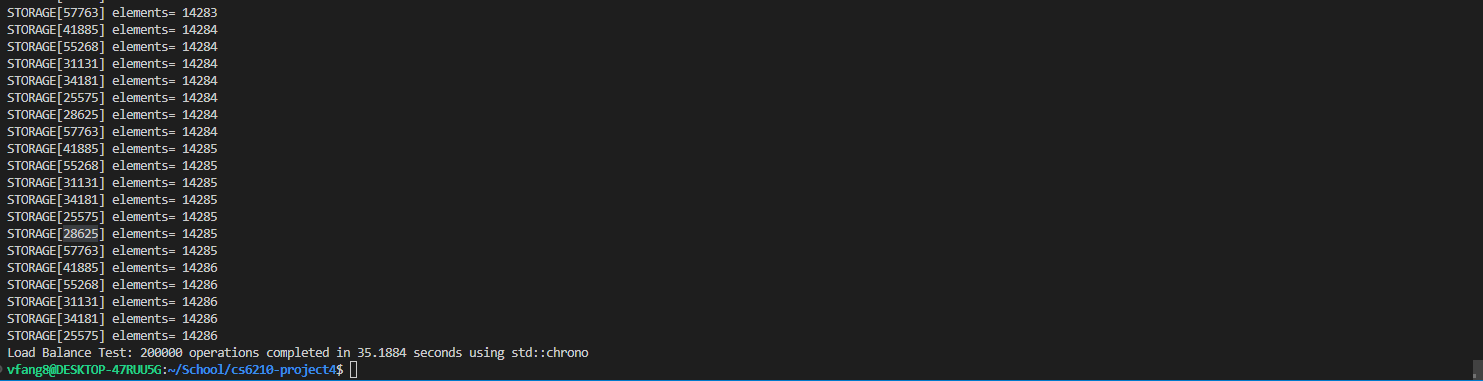
\includegraphics[width=\linewidth]{img/load71.png}\\\\

Here we see a printout of every storage node's size as a put is called. We look here at the last 7 lines of the test output. This corresponds to 7 nodes in 7 unique
storage groups. Note that the sum of the last 7 lines is 100k, matching our 100k puts. We see that they are within 1 of each other, 
indicating our round robin load balancing scheme functions

Below is a histogram of the results:\\\\
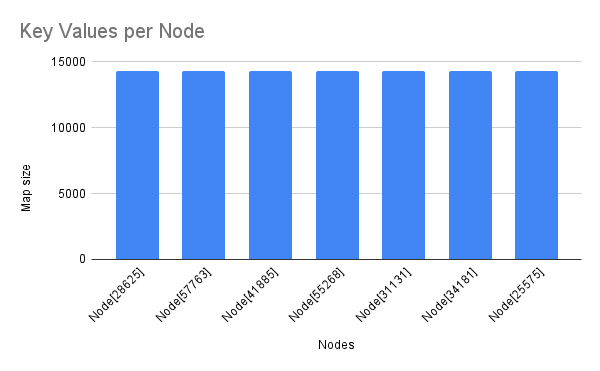
\includegraphics[width=\linewidth]{img/LoadChart.png} 


\end{document}
